\documentclass[11pt]{article}

\usepackage{amssymb}
\usepackage{amsmath}
\usepackage{setspace}
\usepackage{graphicx}
\usepackage{subfig}
\usepackage{color}
\usepackage[left=1.2in, right=1in, top=1in, bottom=1in]{geometry}
\usepackage{verbatim}
\usepackage{hyperref}


\begin{document}

\title{Xoptfoil Example Cases}
\date{\today}
\maketitle

Two example input files are included to accompany this document: ``inputs.txt'' and
``inputs\_withflap.txt.'' The first case is designed to minimize drag at 5 specified lift
coefficients without using flaps. The second case is identical, except that a flap is
included with the hinge at the 75\% chord location. The flap deflection is set to 0 for
the first 3 operating points and optimized for the last two. Sample results are presented
in the following table and figures.
Due to randomness that is naturally present in the optimization algorithms, your
results may not be exactly the same as these, but they will likely be similar.

\begin{table}[!ht]
\centering
\caption{Optimization results}
\begin{tabular}{c c c c c} \\ \hline\hline
Airfoil         & Thickness & Max thickness x/c & Camber & Max camber x/c \\ \hline
Seed            & 10.0\%    & 0.30              & 0.029  & 0.41           \\
Opt - no flap   & 11.3\%    & 0.28              & 0.023  & 0.37           \\
Opt - with flap & 10.9\%    & 0.28              & 0.018  & 0.34           \\
\end{tabular}
\label{table:results}
\end{table}

\begin{figure}[!h]
	\centering
	\subfloat[Opt - no flap]{
		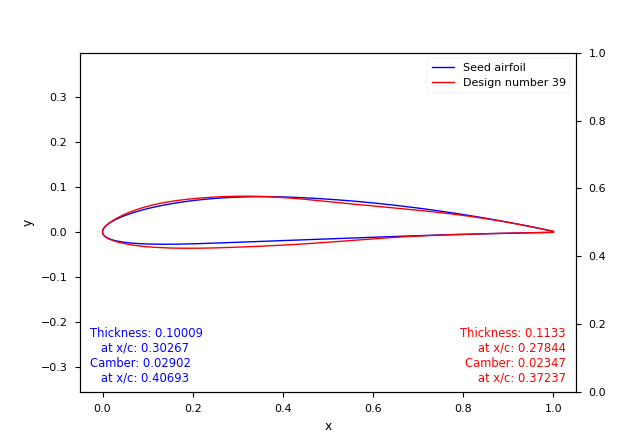
\includegraphics[width=0.49\textwidth]{example_case_figs/case_1_39_coordinates.png}}
	\subfloat[Opt - with flap]{
		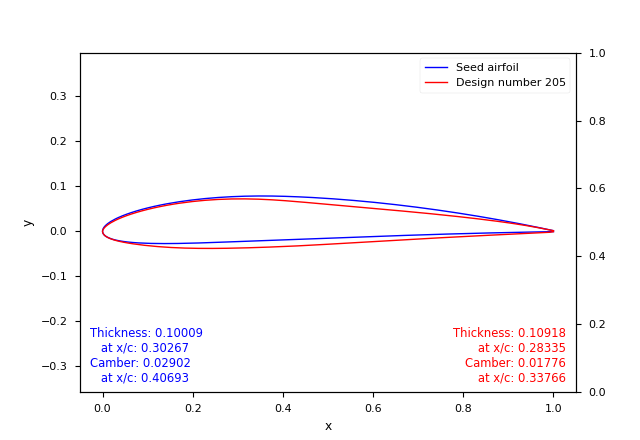
\includegraphics[width=0.49\textwidth]{example_case_figs/case_2_205_coordinates.png}}
	\caption{Seed and optimized airfoils.}
	\label{fig:airfoil}
\end{figure}

\begin{figure}[!h]
	\centering
	\subfloat[Opt - no flap]{
		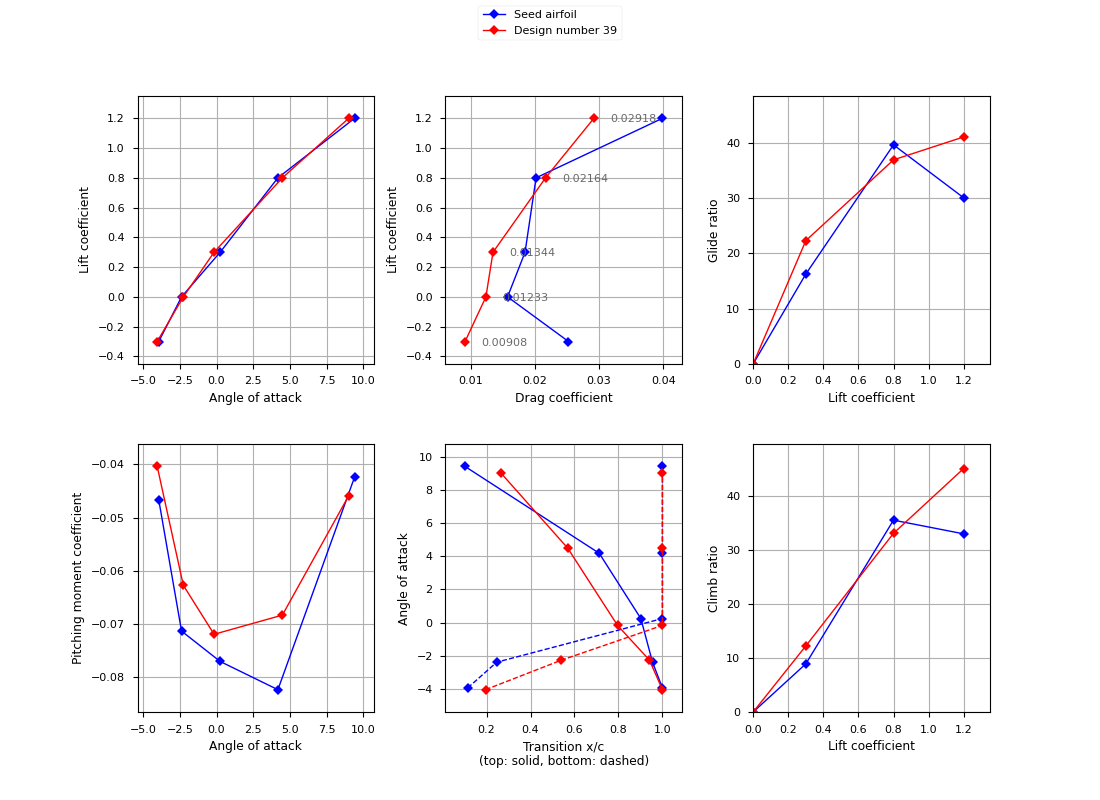
\includegraphics[width=0.49\textwidth]{example_case_figs/case_1_39_polars.png}}
	\subfloat[Opt - with flap]{
		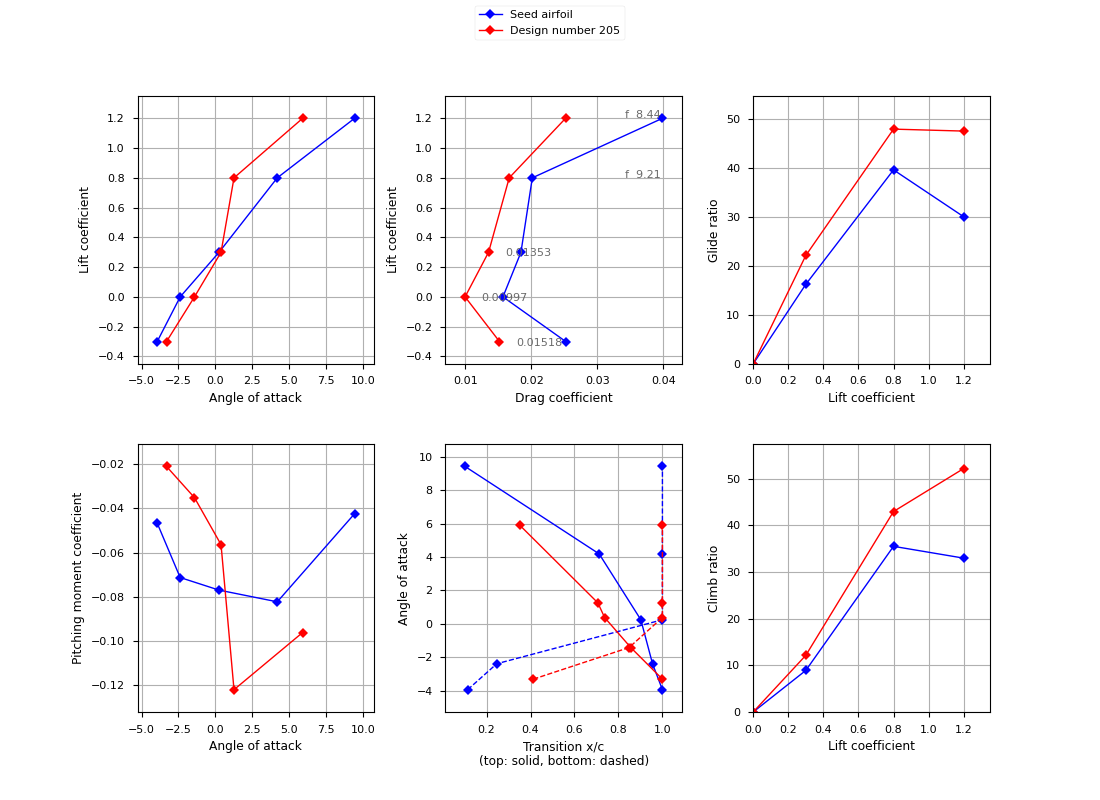
\includegraphics[width=0.49\textwidth]{example_case_figs/case_2_205_polars.png}}
	\caption{Polars for seed and optimized airfoils.}
	\label{fig:polars}
\end{figure}

\begin{figure}[!h]
	\centering
	\subfloat[Opt - no flap]{
		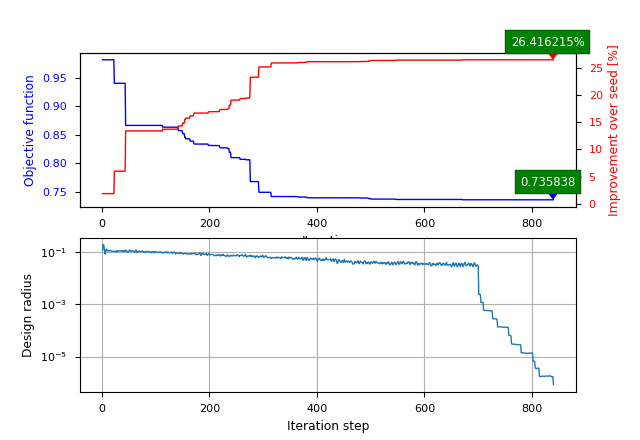
\includegraphics[width=0.49\textwidth]{example_case_figs/case_1_optimization_history.png}}
	\subfloat[Opt - with flap]{
		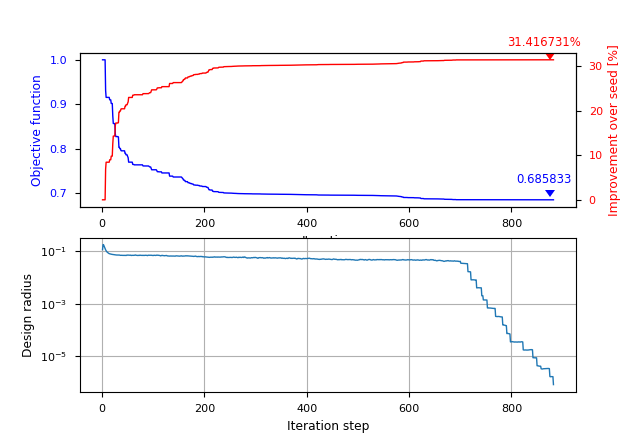
\includegraphics[width=0.49\textwidth]{example_case_figs/case_2_optimization_history.png}}
	\caption{Optimization history.}
	\label{fig:history}
\end{figure}

\end{document}
